\documentclass[a4paper,11pt]{article}
\usepackage{ctex}
\usepackage{enumerate}
\usepackage{times}
\usepackage{mathptmx}
\usepackage{amsmath}
\usepackage{amssymb}
\usepackage{tikz}
\usepackage[top=2cm, bottom=2cm, left=2cm, right=2cm]{geometry}

%\allowdisplaybreaks[4]
\renewcommand{\labelenumi}{\textbf{\emph{\alph{enumi}}.}}
\begin{document}
  \title{����~2-5~��ҵ}
  \author{��������ۿԴ \and ѧ�ţ�161240004}
  \date{}
  \maketitle

  \section{[CS] Problem 5.1-6}
  \begin{enumerate}
    \item $\{(P,P), (P,N), (P,D), (N,P), (N,D), (D,P), (D, N)\}$ \\
    Weights: \\
    $(P,P), (P,N), (P,D), (N,P), (D,P)$: 1/6; \\
    $(N,D), (D,N)$: 1/12.
    \item $P(\text{getting 11 cents}) = P(\{(P,D), (D,P)\}) = 1/3$.
  \end{enumerate}

  \section{[CS] Problem 5.1-10}
  \noindent (A standard deck of playing cards refers to a standard 52-card deck, excluding jokers; 10-J-Q-K-A, A-2-3-4-5 are both straights, but hands such as J-Q-K-A-2 are not, as is commonly acknowledged) \par
  Using five-element sets as model. The sample space $S$ is all the five-element subsets of the 52 cards, and $|S| = \begin{pmatrix} 52 \\ 5 \end{pmatrix}$. $P$ is the uniform probability measure defined on $S$. The event $E$ is the set of all the elements of $S$ which are straights, and we have $|E| = 4^5 \times 10$. Therefore, the probability that a five-card hand is a straight is
  $$P(E) = \frac{|E|}{|S|} = \frac{10,240}{2,598,960} = \frac{128}{32,487} \approx 0.00394$$ \par
  Using five-element permutations as model. The sample space $S$ is all the five permutations of the 52 cards, and $|S| = 52^{\underline{5}}$. $P$ is the uniform probability measure defined on $S$. The event $E$ is the set of all the elements of $S$ which are straights, and we have $|E| = 4^5 \times 10 \times 5!$. Therefore, the probability that a five-card hand is a straight is
  $$P(E) = \frac{|E|}{|S|} = \frac{1,228,800}{311,875,200} = \frac{128}{32,487} \approx 0.00394$$ \par
  The answers are same by using two different models.

  \section{[CS] Problem 5.1-11}
  We use $T$ or $F$ to represent whether or not he answers a single question correctly. The sample space $S$ is $\{T,F\}^{10}$, and we assume that the weights of all the outcomes are the same, i.e. $P$ is the uniform probability measure defined on $S$. Each problem is worth 10 points. \par
  The event that the student gets a score of 80 or higher is $E_1$, and $|E_1| = 1 + 10 + 10 \times 9/2 = 56$. So the probability is
  $$P(E_1) = \frac{|E_1|}{|S|} = \frac{56}{1024} = \frac{7}{128} \approx 0.0547$$ \par
  The event $E_2$ that the student gets a score of 70 or lower is the complement of $E_1$, therefore
  $$P(E_2) = 1 - P(E_1) = 1 - \frac{7}{128} = \frac{121}{128} \approx 0.945$$

  \section{[CS] Problem 5.1-12}
  Let $S, C, T$ represent square, circle and triangle respectively. The sample space $S$ is $\{S, C, T\}^2$.  The event $E$, is $\{SS,CC,TT\}$ ($SS$ stands for $(S,S)$, the same below). The probability that the two shapes on the top are the same is
  $$ P(E) = P(SS) + P(CC) + P(TT) = \frac{1}{36} + \frac{1}{9} + \frac{1}{4} = \frac{7}{18} \approx 0.389 $$

  \section{[CS] Problem 5.1-13}
  For Event 1, the sample space $S_1$ is the set of all two-element subsets of the 13 spades. $P$ is the uniform probability measure defined on $S_1$. The event $E_1$ is $\{\{\spadesuit \text{A}, \spadesuit \text{K}\}\}$. The probability of Event 1 is
  $$ P(E_1) = \frac{|E_1|}{|S_1|} =  \frac{1}{13\times12/2} = \frac{1}{78} \approx 0.0128 $$ \par
  For Event 2, the sample space $S_2$ is the set of all two-element subsets of all 52 cards. $P$ is the uniform probability measure defined on $S_2$. The event $E_1$ is the sets of all two-element sets of an ace and a king. The probability of Event 2 is
  $$ P(E_2) = \frac{|E_2|}{|S_2|} =  \frac{4 \times 4}{52 \times 51 /2} = \frac{8}{663} \approx 0.0121 $$ \par
    Therefore, the two events are not equally likely.

  \section{[CS] Problem 5.2-2}
  Let $E, F$ represent the events that $\spadesuit \text{K}$ or $\spadesuit \text{Q}$ is selected, respectively. The event that the king or queen of spades is among the cards selected is $E \cup F$. Therefore, the probability is
  $$ P(E \cup F) = P(E)+P(F)-P(E\cap F) = \frac{7}{28} + \frac{7}{28} - \frac{1}{28} = \frac{15}{28} \approx 0.536$$

  \section{[CS] Problem 5.2-9}
  The sample space $S$ is the set of all possible arrangements, and $|S|=n!$. Let $E_i$ denote the event that the $i$-th person who gets the letter intended for him or her. Then, by inclusion-exclusion principle, we have
  \begin{align*}
    \left| \bigcup_{i=1}^{n} E_i \right| &= \sum_{k=1}^{n}(-1)^{k+1} \sum_{\substack{i_1, i_2, \cdots i_k: \\ 1 \leq i_1 < i_2 < \cdots < i_k \leq n }} \left| \bigcap_{j=1}^k E_{i_j}\right| \\
    &= \sum_{k=1}^{n}(-1)^{k+1}\begin{pmatrix}n\\k\end{pmatrix}(n-k)! \\
    &= \sum_{k=1}^{n}(-1)^{k+1}\frac{n!}{k!} \\
  \end{align*}
  Hence, the number of ways that nobody gets the correct letter is
  \begin{align*}
    n!-\left|\bigcup_{i=1}^{n} E_i\right| = \sum_{k=0}^{n}(-1)^{k}\frac{n!}{k!} \\
  \end{align*}
  And the probability $P(E)$ is
  $$ P(E) = \sum_{k=0}^{n}(-1)^{k}\frac{n!}{k!} / n! = \sum_{k=0}^{n}(-1)^{k}\frac{1}{k!} $$

  \section{[CS] Problem 5.2-10}
  The sample space $S=\{L_1,L_2,\cdots,L_k\}^n$, and $|S| = k^n$. Let $E_i$ represent the event that there is no key in the $i$-th location. For $i_1 < i_2 < \cdots < i_j$, we have
  $$\left| \bigcap_{l=1}^j E_{i_l} \right| = (k-j)^n$$ \par
  By inclusion-exclusion principle, we have
  $$\left| \bigcup_{i=1}^{k} E_i \right| = \sum_{j=1}^{k} (-1)^{j+1} \sum_{\substack{i_1,i_2,\cdots,i_j: \\ 1 \leq i_1 < i_2 < \cdots < i_j \leq k}} \left| \bigcap_{l=1}^j E_{i_l} \right| = \sum_{j=1}^{k} (-1)^{j+1} \begin{pmatrix} k \\ j \end{pmatrix} (k-j)^n $$
  Hence, the number of cases that every location gets at least one key is
  $$ k^n - \sum_{j=1}^{k} (-1)^{j+1} \begin{pmatrix} k \\ j \end{pmatrix} (k-j)^n = \sum_{i=0}^{k} (-1)^{i} \begin{pmatrix} k \\ i \end{pmatrix} (k-i)^n $$
  And the probability $P(E)$ is
  $$ P(E) = \frac{\sum_{i=0}^{k} (-1)^{i} \begin{pmatrix} k \\ i \end{pmatrix} (k-i)^n}{k^n} $$

  \section{[CS] Problem 5.2-14}
  Let the sample space $S$ be the set of all possible circular permutations, and $|S|=(2n-1)!$. Let $E_i$ represent the event that the $i$-th couple are side-by-side. For $i_1 < i_2 < \cdots < i_k$, we have
  $$\left| \bigcap_{j=1}^k E_{i_j} \right| = (2n-k-1)!2^k$$ \par
  By inclusion-exclusion principle, we have
  $$\left| \bigcup_{i=1}^{n} E_i \right| = \sum_{j=1}^{n} (-1)^{j+1} \sum_{\substack{i_1,i_2,\cdots,i_j: \\ 1 \leq i_1 < i_2 < \cdots < i_j \leq n}} \left| \bigcap_{l=1}^j E_{i_l} \right| = \sum_{i=1}^{n} (-1)^{i+1} \begin{pmatrix} n \\ i \end{pmatrix} (2n-i-1)!2^i$$
  The number of circular permutations that no husband and wife are side-by-side is
  $$(2n-1)!-\sum_{i=1}^{n} (-1)^{i+1} \begin{pmatrix} n \\ i \end{pmatrix} (2n-i-1)!2^i = \sum_{i=0}^{n} (-1)^{i} \begin{pmatrix} n \\ i \end{pmatrix} (2n-i-1)!2^i $$
  The probability $P(E)$ is
  $$ P(E) = \frac{\sum_{i=0}^{n} (-1)^{i} \begin{pmatrix} n \\ i \end{pmatrix} (2n-i-1)!2^i}{(2n-1)!} $$

  \section{[CS] Problem 5.2-15}
  Let $C$ be the set of all these $m$ objects. Let $E_i$ be the set of objects which have the $i$-th property. By inclusion-exclusion principle, we have
  $$\left| \bigcup_{i=1}^{p} E_i \right| = \sum_{j=1}^{p} (-1)^{j+1} \sum_{\substack{i_1,i_2,\cdots,i_j: \\ 1 \leq i_1 < i_2 < \cdots < i_j \leq p}} \left| \bigcap_{l=1}^j E_{i_l} \right| = \sum_{i=1}^{p} (-1)^{i+1} \sum_{K: K \subseteq P, |K| = i} N_a(K)$$
  And we know that $C = N_a(\varnothing)$. Therefore,
  $$N_e(\varnothing) = |C| - \left| \bigcup_{i=1}^{p} E_i \right| = \sum_{i=0}^{|P|} (-1)^{i} \sum_{K: K \subseteq P, |K| = i} N_a(K) =  \sum_{K: K \subseteq P}(-1)^{|K|} N_a(K)$$ \par
  Explanation: For each element $b$ in $B$, we define a property $b$ for the functions. A function $f$ has the property $b$ if and only if for every $a \in A$, $(a, b) \notin f$. $N_a(K)$ means the number of the functions from $A$ to $B ~\backslash~ K$, i.e. $N_a(K) = (|B|-|K|)^{|A|}$. $N_e(\varnothing)$ means the number of the onto functions, and
  $$ N_e(\varnothing) = \sum_{K: K \subseteq P}(-1)^{|K|} N_a(K) = \sum_{i=0}^{|B|} (-1)^i \begin{pmatrix} |B| \\ i \end{pmatrix} (|B|-i)^{|A|}$$ \par
  Application to Problem 9: Define $n$ properties for the arrangements. The $i$-th property means that the $i$-th person gets the correct letter. The sample $S$ is the set of all possible arrangements, and $|S| = n!$. The event $E$ is that nobody gets the correct letter, and we have
  $$ |E| = N_e(\varnothing) = \sum_{K:K \in P} (-1)^{|K|}N_a(K) =\sum_{i=0}^{n}(-1)^{i}\begin{pmatrix} n \\ i \end{pmatrix}(n-i)! = \sum_{i=0}^{n}(-1)^{i}\frac{n!}{i!} $$
  Therefore, the probability is
  $$ P(E) = |E|/n! = \sum_{i=0}^{n}(-1)^{i}\frac{1}{i!} $$

  \section{[CS] Problem 5.3-3}
  Let the sample space $S = \{T,F\}^3$, and $|S| = 8$. $P$ is the uniform probability measure defined on $S$. Let $E_1$ denote the event of at most one tail, i.e. $E_1 = \{FFF, TFF, FTF, FFT\}$, $E_2$ denote the event that all not all flips are identical, i.e. $E_2 = \{TFF, FTF, FFT, TTF, TFT, FTT\}$. Calculate the probability of these events:
  $$ P(E_1) = \frac{|E_1|}{|S|} = \frac{1}{2} = 0.5 $$
  $$ P(E_2) = \frac{|E_2|}{|S|} = \frac{3}{4} = 0.75 $$
  $$ P(E_1 \cap E_2) = \frac{|E_1 \cap E_2|}{|S|} = \frac{3}{8} = 0.375 $$ \par
  Since $P(E_1 \cap E_2) = P(E_1) P(E_2)$, by product principle for independent probabilities, the two events are independent.

  \section{[CS] Problem 5.3-4}
  The sample space $S=\{1,2,3,4,5,6\}^2$, and $P$ is the uniform probability measure defined on $S$. \par
  Let $E_{1,i}$ denote the event that ``$i$ dots are on top of the first die'', i.e. $E_{1,i} = \{i1,i2,i3,i4,i5,i6\}$, and $E_{2,j}$ denote the event that ``$j$ dots are on top of the second die'' likewise. Therefore
  $$ P(E_{1,i}) = \frac{|E_{1,i}|}{|S|} = \frac{1}{6} $$
  $$ P(E_{2,j}) = \frac{|E_{2,j}|}{|S|} = \frac{1}{6} $$
  $$ P(E_{1,i} \cap E_{2,j}) = \frac{|E_{1,i} \cap E_{2,j}|}{|S|} = \frac{|\{ij\}|}{|S|} = \frac{1}{36} $$
  Since, $P(E_{1,i})P(E_{2,j}) = P(E_{1,i} \cap E_{2,j})$, the two events are independent.

  \section{[CS] Problem 5.3-8}
  Let the sample space $S$ be the set of all 13-element subset of the 52 cards. Let $E_1$ denote the event that a bridge hand has four aces, $E_2$ denote the event that it has at least one ace, $E_3$ denote the event that it has the ace of spades. $P$ is the uniform probability measure defined on $S$. Calculate the probabilities:
  $$ P(E_1) = \frac{|E_1|}{|S|} = \begin{pmatrix} 48 \\ 9 \end{pmatrix} / \begin{pmatrix} 52 \\ 13 \end{pmatrix} = \frac{11}{4165} \approx 0.00264 $$
  $$ P(E_2) = 1 - \frac{|S~\backslash~E_2|}{|S|} = 1 - \begin{pmatrix} 48 \\ 13 \end{pmatrix} / \begin{pmatrix} 52 \\ 13 \end{pmatrix} = \frac{14,498}{20,825} \approx 0.696 $$
  $$ P(E_3) = 1 - \frac{|S~\backslash~E_3|}{|S|} = 1 - \begin{pmatrix} 51 \\ 13 \end{pmatrix} / \begin{pmatrix} 52 \\ 13 \end{pmatrix} = \frac{1}{4} = 0.25 $$ \par
  Therefore
  $$ P(E_1|E_2) = \frac{|E_1 \cap E_2|}{|E_2|} = \frac{|E_1|}{|E_2|} = \frac{5}{1316} \approx 0.00379$$
  $$ P(E_1|E_3) = \frac{|E_1 \cap E_3|}{|E_3|} = \frac{|E_1|}{|E_3|} = \frac{44}{4165} \approx 0.01056$$
  The latter one is larger.

  \section{[CS] Problem 5.3-11}
  $E$ and $F$ are independent if and only if $P(E \cap F) = P(E) P(F)$. Since $E \cap F = \varnothing$, $E$ and $F$ are independent if and only if $P(E) = 0$ or $P(F) = 0$.
  
  \section{[CS] Problem 5.3-12}
  Let $B$ denote a boy, $G$ denote a girl, then the sample space $S = \{BB, BG, GB, GG\}$. Assume every outcome has the same weight, i.e. $P$ is the uniform probability measure. \par
  Let $E_1$ be the event that the family has two girls, $E_2$ be the event that one of the children is a girl. We have $P(E_1)=0.25$, $P(E_2)=0.75$, therefore
  $$P(E_1|E_2) = \frac{P(E_1 \cap E_2)}{P(E_2)} = \frac{P(E_1)}{P(E_2)} = \frac{1}{3} $$
  Let $E_3$ be the event that the children are both boys, $E_4$ be the event that the older child is a boy. We have $P(E_3)=0.25$, $P(E_4)=0.5$, therefore
  $$P(E_3|E_4) = \frac{P(E_3 \cap E_4)}{P(E_4)} = \frac{P(E_3)}{P(E_4)} = 0.5$$
  
  \section{[CS] Problem 5.3-13}
  Let $A$, $B$, $C$ denote the three curtains. The first step of this process is to determine a curtain behind which is a new car randomly. The second step is that you pick a curtain randomly. The third step is that the emcee rules out a curtain that you didn't pick randomly. We use a tree diagram to illustrate the whole process. \\[0.2cm]
  %\scriptsize
  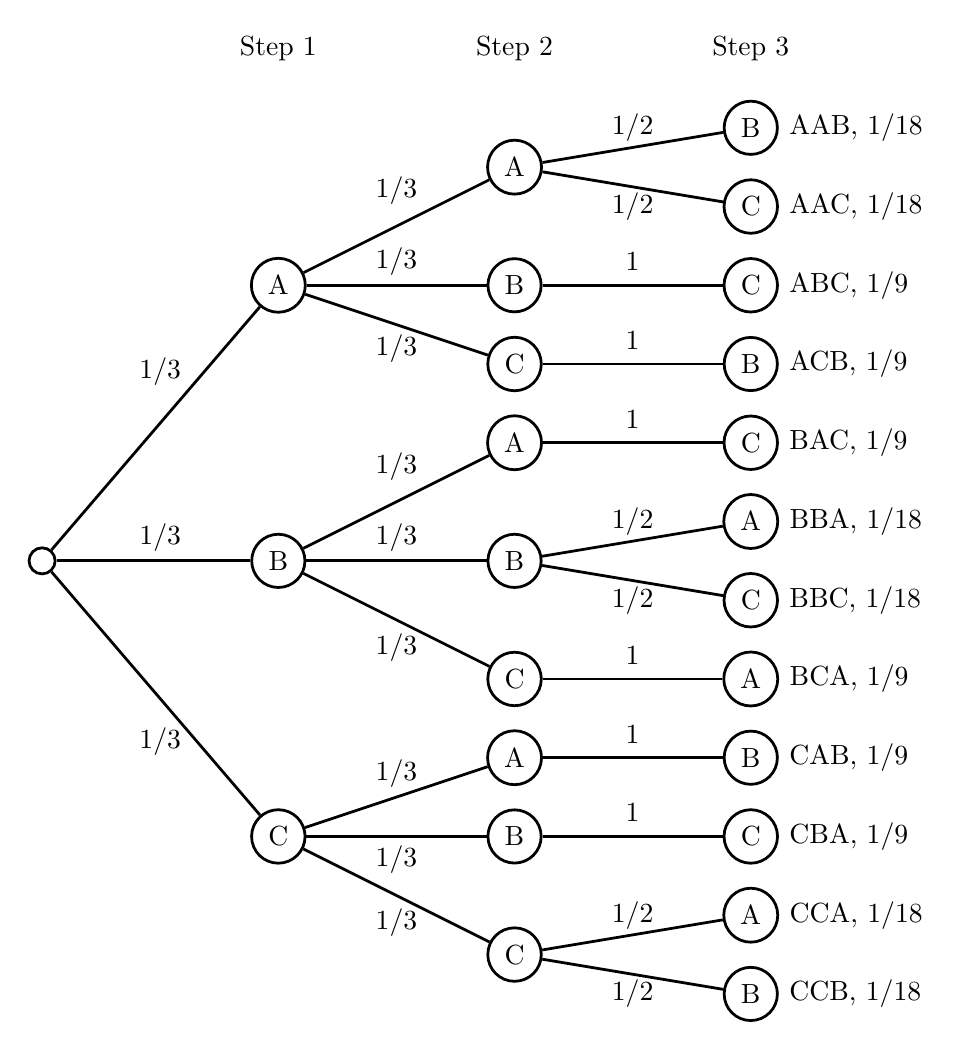
\begin{tikzpicture}[line width = 1pt,
                    solid/.style = {circle, draw, fill = black, minimum size = 0.3cm},
                    empty/.style = {circle, draw, fill = white, minimum size = 0.3cm}]
  \node at (3,-1)[align=center]{Step 1};
  \node at (6,-1)[align=center]{Step 2};
  \node at (9,-1)[align=center]{Step 3};
  \node [empty] (T01) at (0,-7.5) {};
  \node [empty] (T11) at (3,-4) {A};
  \node [empty] (T12) at (3,-7.5) {B};
  \node [empty] (T13) at (3,-11) {C};
  \node [empty] (T21) at (6,-2.5) {A};
  \node [empty] (T22) at (6,-4) {B};
  \node [empty] (T23) at (6,-5) {C};
  \node [empty] (T24) at (6,-6) {A};
  \node [empty] (T25) at (6,-7.5) {B};
  \node [empty] (T26) at (6,-9) {C};
  \node [empty] (T27) at (6,-10) {A};
  \node [empty] (T28) at (6,-11) {B};
  \node [empty] (T29) at (6,-12.5) {C};
  \node [empty, label = right:{AAB, 1/18}] (T31) at (9,-2) {B};
  \node [empty, label = right:{AAC, 1/18}] (T32) at (9,-3) {C};
  \node [empty, label = right:{ABC, 1/9}] (T33) at (9,-4) {C};
  \node [empty, label = right:{ACB, 1/9}] (T34) at (9,-5) {B};
  \node [empty, label = right:{BAC, 1/9}] (T35) at (9,-6) {C};
  \node [empty, label = right:{BBA, 1/18}] (T36) at (9,-7) {A};
  \node [empty, label = right:{BBC, 1/18}] (T37) at (9,-8) {C};
  \node [empty, label = right:{BCA, 1/9}] (T38) at (9,-9) {A};
  \node [empty, label = right:{CAB, 1/9}] (T39) at (9,-10) {B};
  \node [empty, label = right:{CBA, 1/9}] (T310) at (9,-11) {C};
  \node [empty, label = right:{CCA, 1/18}] (T311) at (9,-12) {A};
  \node [empty, label = right:{CCB, 1/18}] (T312) at (9,-13) {B};
  
  \node at (1.5,-5.1) {1/3};
  \node at (1.5,-7.2) {1/3};
  \node at (1.5,-9.8) {1/3};
  \draw (T01)--(T11);
  \draw (T01)--(T12);
  \draw (T01)--(T13);
  
  \node at (4.5,-2.8) {1/3};
  \node at (4.5,-3.7) {1/3};
  \node at (4.5,-4.8) {1/3};
  \node at (4.5,-6.3) {1/3};
  \node at (4.5,-7.2) {1/3};
  \node at (4.5,-8.6) {1/3};
  \node at (4.5,-10.2) {1/3};
  \node at (4.5,-11.3) {1/3};
  \node at (4.5,-12.1) {1/3};
  \draw (T11)--(T21);
  \draw (T11)--(T22);
  \draw (T11)--(T23);
  \draw (T12)--(T24);
  \draw (T12)--(T25);
  \draw (T12)--(T26);
  \draw (T13)--(T27);
  \draw (T13)--(T28);
  \draw (T13)--(T29);
  
  \node at (7.5,-2) {1/2};
  \node at (7.5,-3) {1/2};
  \node at (7.5,-3.7) {1};
  \node at (7.5,-4.7) {1};
  \node at (7.5,-5.7) {1};
  \node at (7.5,-7) {1/2};
  \node at (7.5,-8) {1/2};
  \node at (7.5,-8.7) {1};
  \node at (7.5,-9.7) {1};
  \node at (7.5,-10.7) {1};
  \node at (7.5,-12) {1/2};
  \node at (7.5,-13) {1/2};
  \draw (T21)--(T31);
  \draw (T21)--(T32);
  \draw (T22)--(T33);
  \draw (T23)--(T34);
  \draw (T24)--(T35);
  \draw (T25)--(T36);
  \draw (T25)--(T37);
  \draw (T26)--(T38);
  \draw (T27)--(T39);
  \draw (T28)--(T310);
  \draw (T29)--(T311);
  \draw (T29)--(T312);
  \end{tikzpicture} \par
  \normalsize
  The sample space $S = \{AAB, AAC, ABC, ACB, BAC, BBA, BBC, BCA, CAB, CBA, CCA, CCB\}$. The weight of each outcome is shown in the diagram. Let $E_1$ be the event that the car is behind the curtain you first chose, i.e. $E_1 = \{AAB, AAC, BBA, BBC, CCA, CCB\}$, $E_2$ be the event that the car is behind the curtain you switch. $E_2$ is the complement of $E_1$. Calculate the probabilities:
  $$ P(E_1) = 6 \times \frac{1}{18} = \frac{1}{3}, \quad P(E_2) = 1 - P(E_2) = \frac{2}{3}$$
  So you'd better switch.
\end{document}
